%%%%%%%%%%%%%%%%%%%%%%%%%%%%%%%%%%%%%%%%%%%%%%%%%%%%%%%%%%%%%%%%%
%  _____       ______   ____									%
% |_   _|     |  ____|/ ____|  Institute of Embedded Systems	%
%   | |  _ __ | |__  | (___    Wireless Group					%
%   | | | '_ \|  __|  \___ \   Zuercher Hochschule Winterthur	%
%  _| |_| | | | |____ ____) |  (University of Applied Sciences)	%
% |_____|_| |_|______|_____/   8401 Winterthur, Switzerland		%
%																%
%%%%%%%%%%%%%%%%%%%%%%%%%%%%%%%%%%%%%%%%%%%%%%%%%%%%%%%%%%%%%%%%%

\chapter{Metastabilität}\label{chap.metastabilitat}

\section{Metastabiler Zustand}\label{sect.meatastabil_def}
Metastabilität bedeutet, dass der Ausgang eines Flip-Flops nicht dem Eingang entsprechen \textit{muss}. In einem metastabilen Zustand kann ein Ausgang korrekt sein, muss aber nicht.
Im Idealfall wählt wählt ein Flip-Flop seinen Ausgangswert selbst (siehe Abbildung \ref{fig.metastabil.schlimmster_Fal} oberes Signal). Im schlechten Fall “hängt” sich das Flip-Flop “auf” und toggelt permanent zwischen '0' und '1' (Abbildung \ref{fig.metastabil.schlimmster_Fal} unteres Signal).

\begin{figure}[H]
	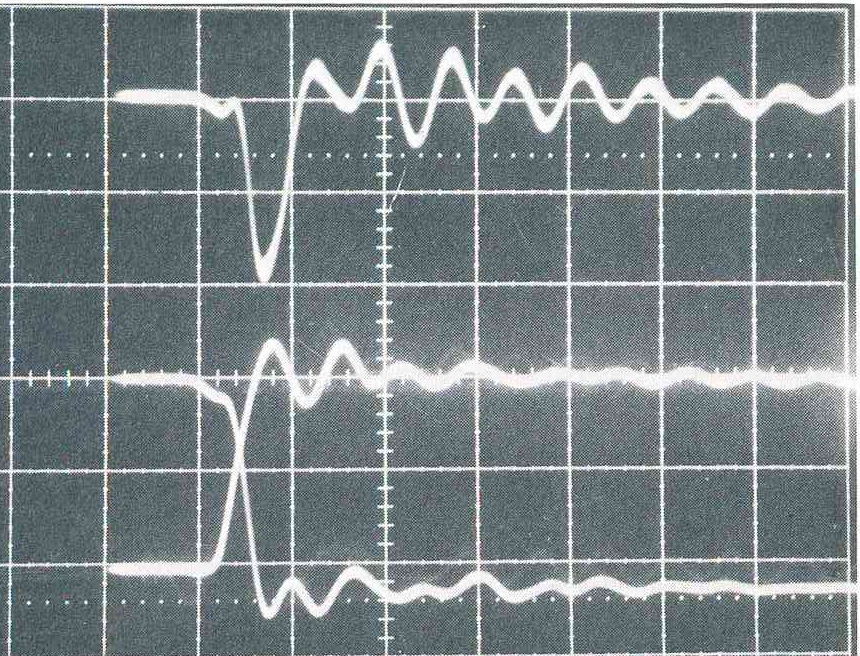
\includegraphics[width=0.4\textwidth]{images/metastability/metastability_2_IO.png}
	\caption{Metastabilität schlimmster Fall \cite{F_metastability}}
	\label{fig.metastabil.schlimmster_Fall}
\end{figure}


\section{Ursache von Metastabilität}\label{sect.meatastabil_ursache}

Die Ursache unsicherer Ausgangswerte liegen darin, dass das Inputsignal eines Flip-Flops zur falschen Zeit wechselt.

\begin{quote}
''If data inputs to a flip-flop are changing at the instant of the clock pulse, a problem known as \textit{metastability} may occur. In the metastable case, the flip-flop does not settle in to a stable state'' \cite{ReferenceManual}
\end{quote}

\begin{quote}
''If the amplitude of the runt pulse is \textit{exactly the treshold level of the SET input of the output cell}, the cell will be driven to its metastable state. The metastable state is the condition that is roughly defined as ''half SET and half RESET'' \cite{F_metastability}
\end{quote}

Trifft der anzulegende Wert zu spät ein wird die \textit{setup time} verletzt und wird der Signalwert zu früh entwendet, verletzt die \textit{hold time}. Metastabilität kann vermieden werden, wenn diese zwei Zeiten strikt eingehalten werden:

\begin{quote}
''Metastabilit is avoided by holding the information stable before and after the clock pulse  for a set period of time, called the setup time for the data line an the hold time for the control line.''\cite{ReferenceManual}
\end{quote}

\begin{figure}[H]
	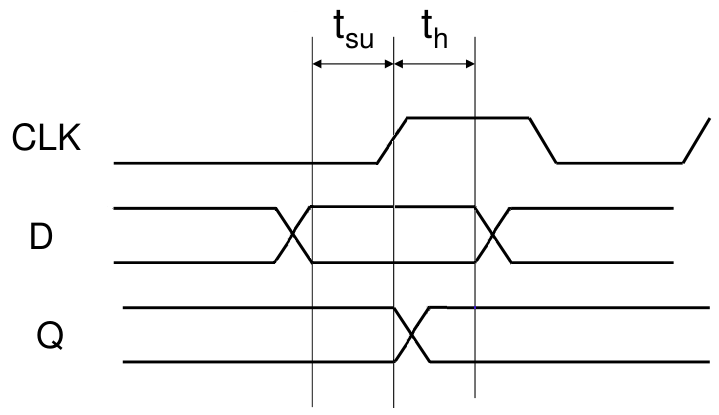
\includegraphics[width=0.4\textwidth]{images/metastability/kritscheZeit_FF.png}
	\caption{Einhalten der Datenzeiten}
	\label{fig.metastabil.kritisches_zeitfenster}
\end{figure}

Um Metastabilität zu vermeiden, sollte die Logik möglichst klein, die Bauteile beieinander und der Systemtakt an die längste Pfadzeit angepasst werden. Der maximal erlaubte Systemtakt kann in quartus mit dem Timequest Time Analyser abgefragt werden.

\section{Metastabilität erzeugen}\label{sect.meatastabil_erzeugen}

\subsection{Konzept}\label{sect.metastabil_ansatz}

Aufgebaut wird ein System mit zwei \textit{clock domains}.  \textit{Clock domain 1}, Gebiet 1 genannt,  beinhaltet einen Zähler, der an die \textit{clock domain 2}, als Gebiet 2 bezeichnet, asynchrone Impulse sendet. Gebiet 2 verarbeitet diese Impulse in einer \textit{finate state machine}. Bei korrekter Funktionsweise wechset die \textit{fsm} zwischen den definierten \textit{states}. Funktioniert sie falsch, fällt die \textit{fsm} in einen \textit{state}, den sie nicht implementiert hat.

\begin{figure}[H]
	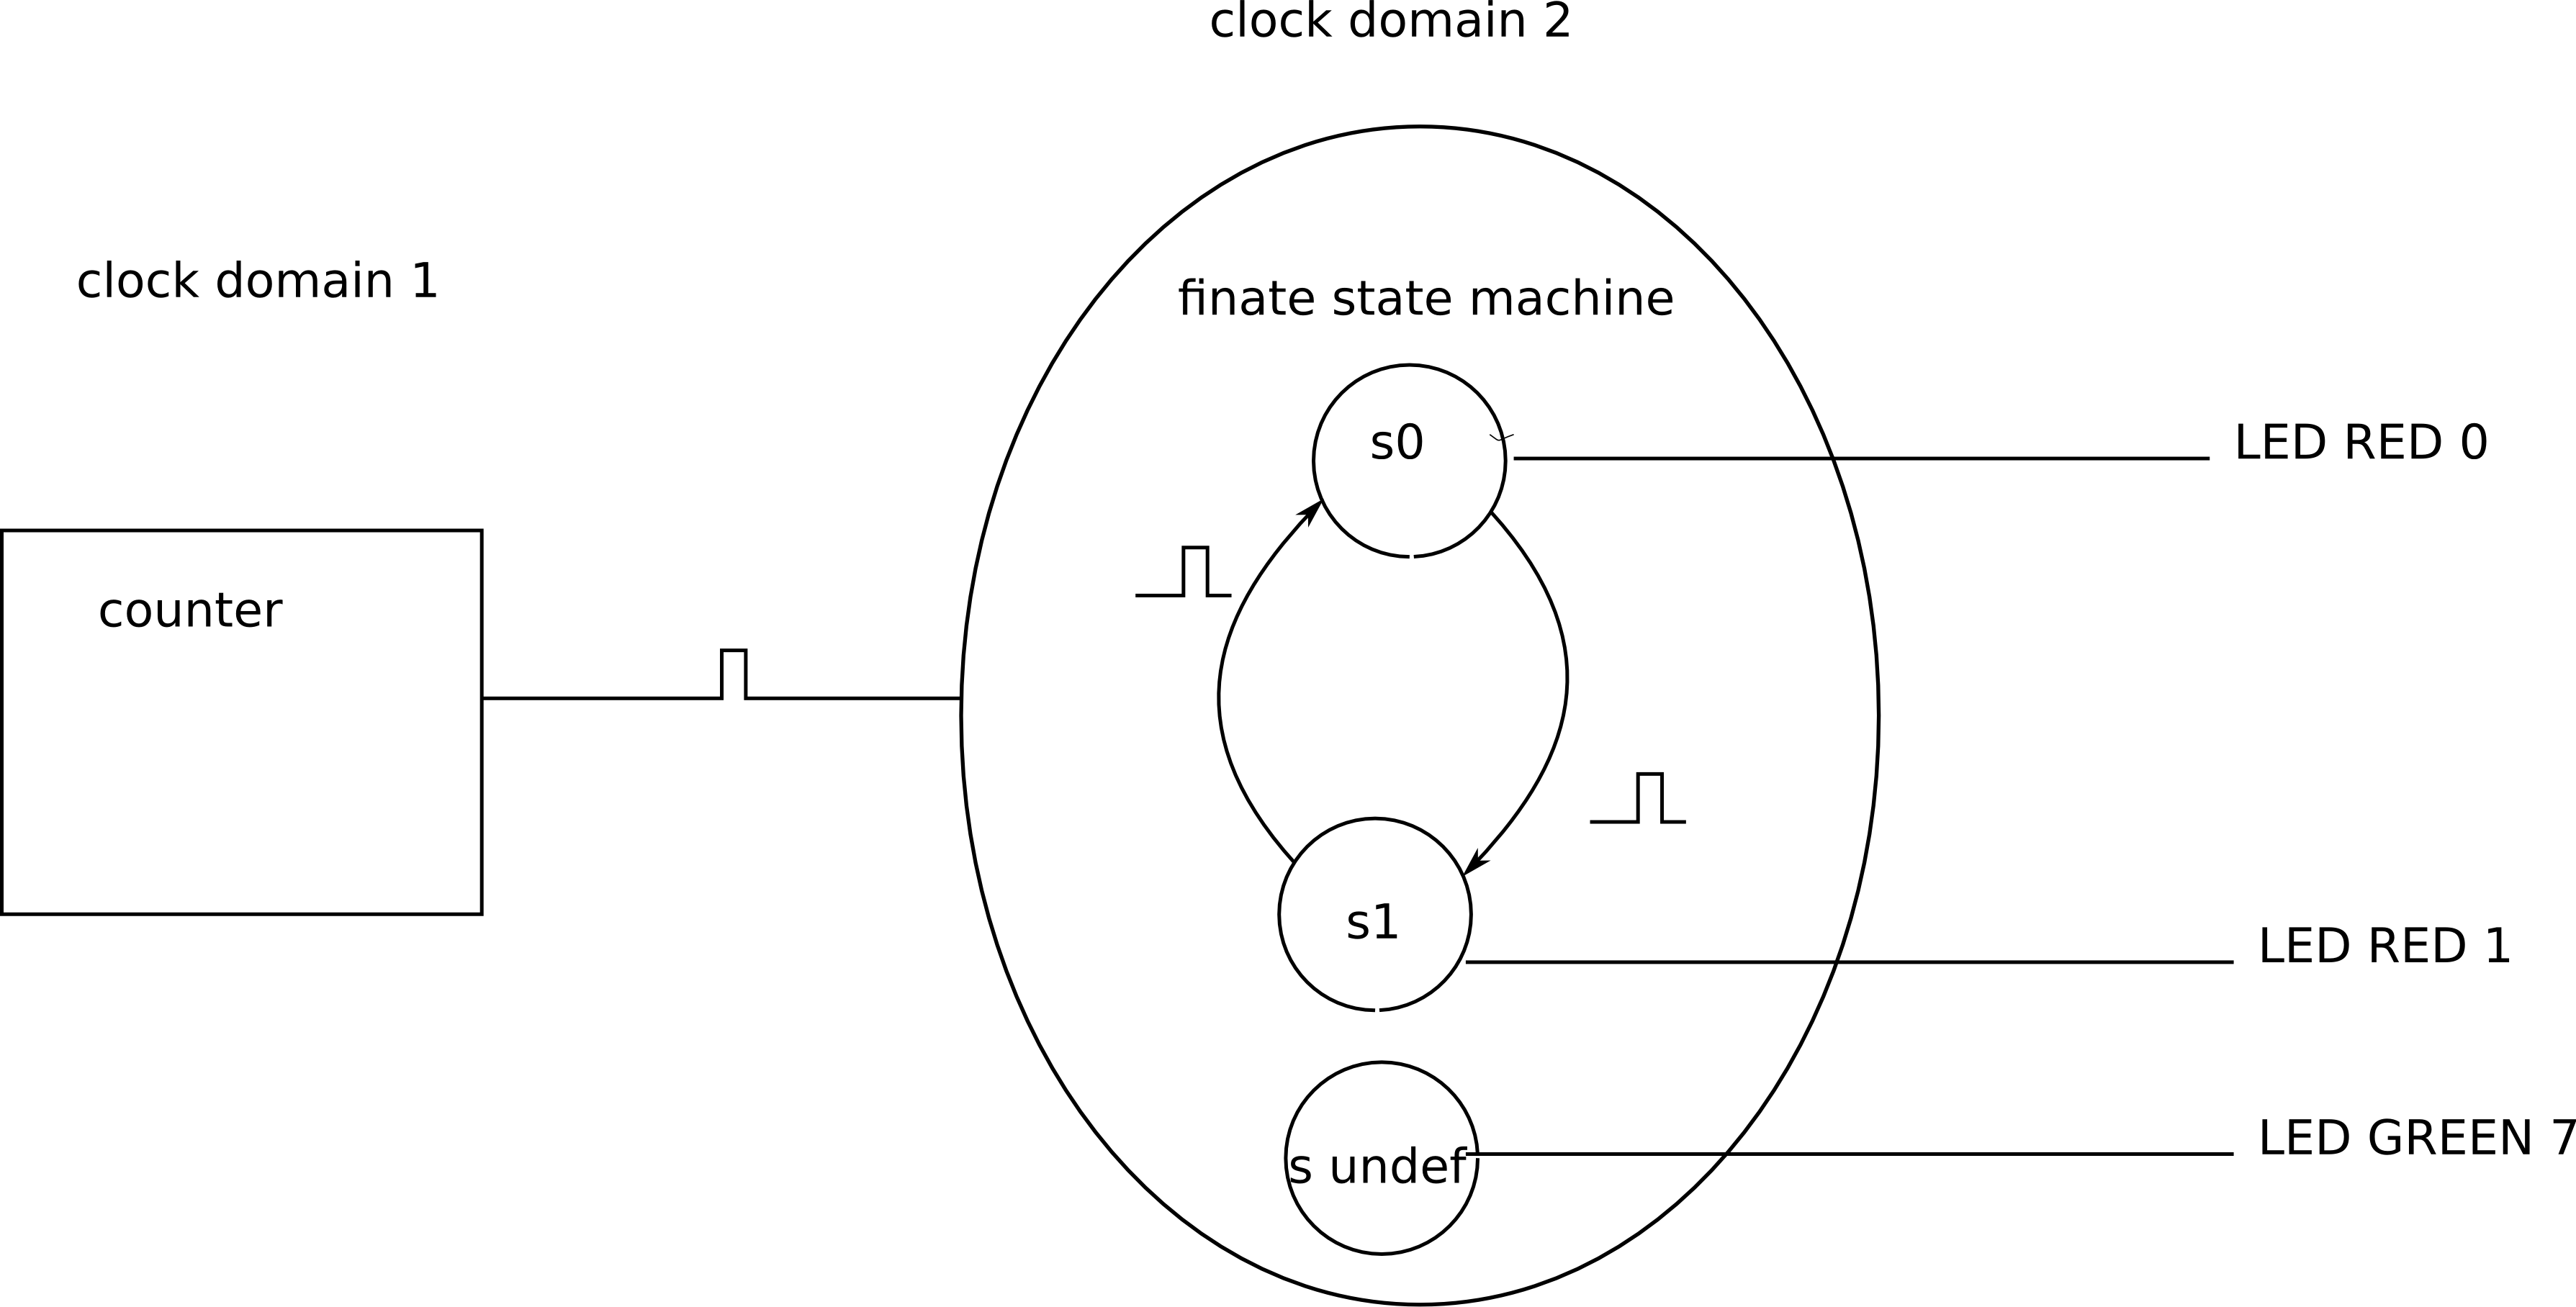
\includegraphics[width=0.8\textwidth]{images/metastability/konzept.png}
	\caption{Konzept Metastabilität nachweisen}
	\label{fig.metastabil.fsm}
\end{figure}

\subsection{Umsetzung}\label{sect.metastabil_implementation}

Als Hardware wird das altera board De2 genommen und mit der Software quartus 13osp0 gearbeitet. Da die zwei Takte nicht Vielfache voneinander sein dürfen, wure für den Zähler ein Takt von 27 MHz und für die \textit{fsm} ein Takt von 50 MHz. Der Takt des Zählers ist leicht schneller als die Hälfte des \textit{fsm}-Taktes und schiebt sich  vorwärts (siehe Abbildung \ref{fig.metastabil.takte}). Das Verletzen der \textit{setup time} ist eine Frage der Zeit.

\begin{figure}[H]
	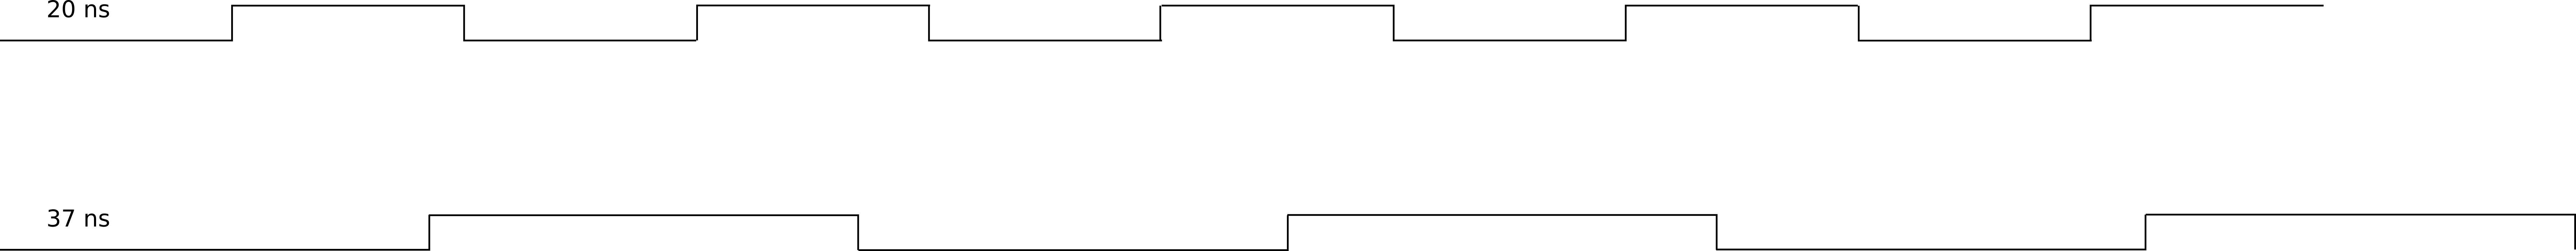
\includegraphics[width=1\textwidth]{images/metastability/2_takte.png}
	\caption{Die zwei Taktzeiten}
	\label{fig.metastabil.takte}
\end{figure}

Die Zustandsüberprüfung erfolgt über das Ausgeben des aktuellen Zustands auf den zwei roten LEDs. 

\begin{itemize}
	\item Zustand = s0\\
	Rote LED 0 ist an
	\item Zustand = s1\\
	 Rote LED 1 ist an
	\item Zustand = \textit{OTHERS}\\
	 Grüne LED 17 ist an\\
\end{itemize}

Funktioniert die \textit{fsm}, blinken die zwei roten LEDs abwechslungsweise. Fällt die \textit{fsm} in einen undefinierten Zustand, leuchtet die grüne LED. Um die Ursache der Metastabilität, das Verletzten der \textit{setup time} zu verhindern, wird eine optionale Synchronisation durch Switch 17 eingebaut. Ist Swicht 17  auf '1', wird der Puls der \textit{clock domain} 27 MHz durch ein Flip-Flop auf 50 MHz synchronisiert.

\begin{figure}[H]
	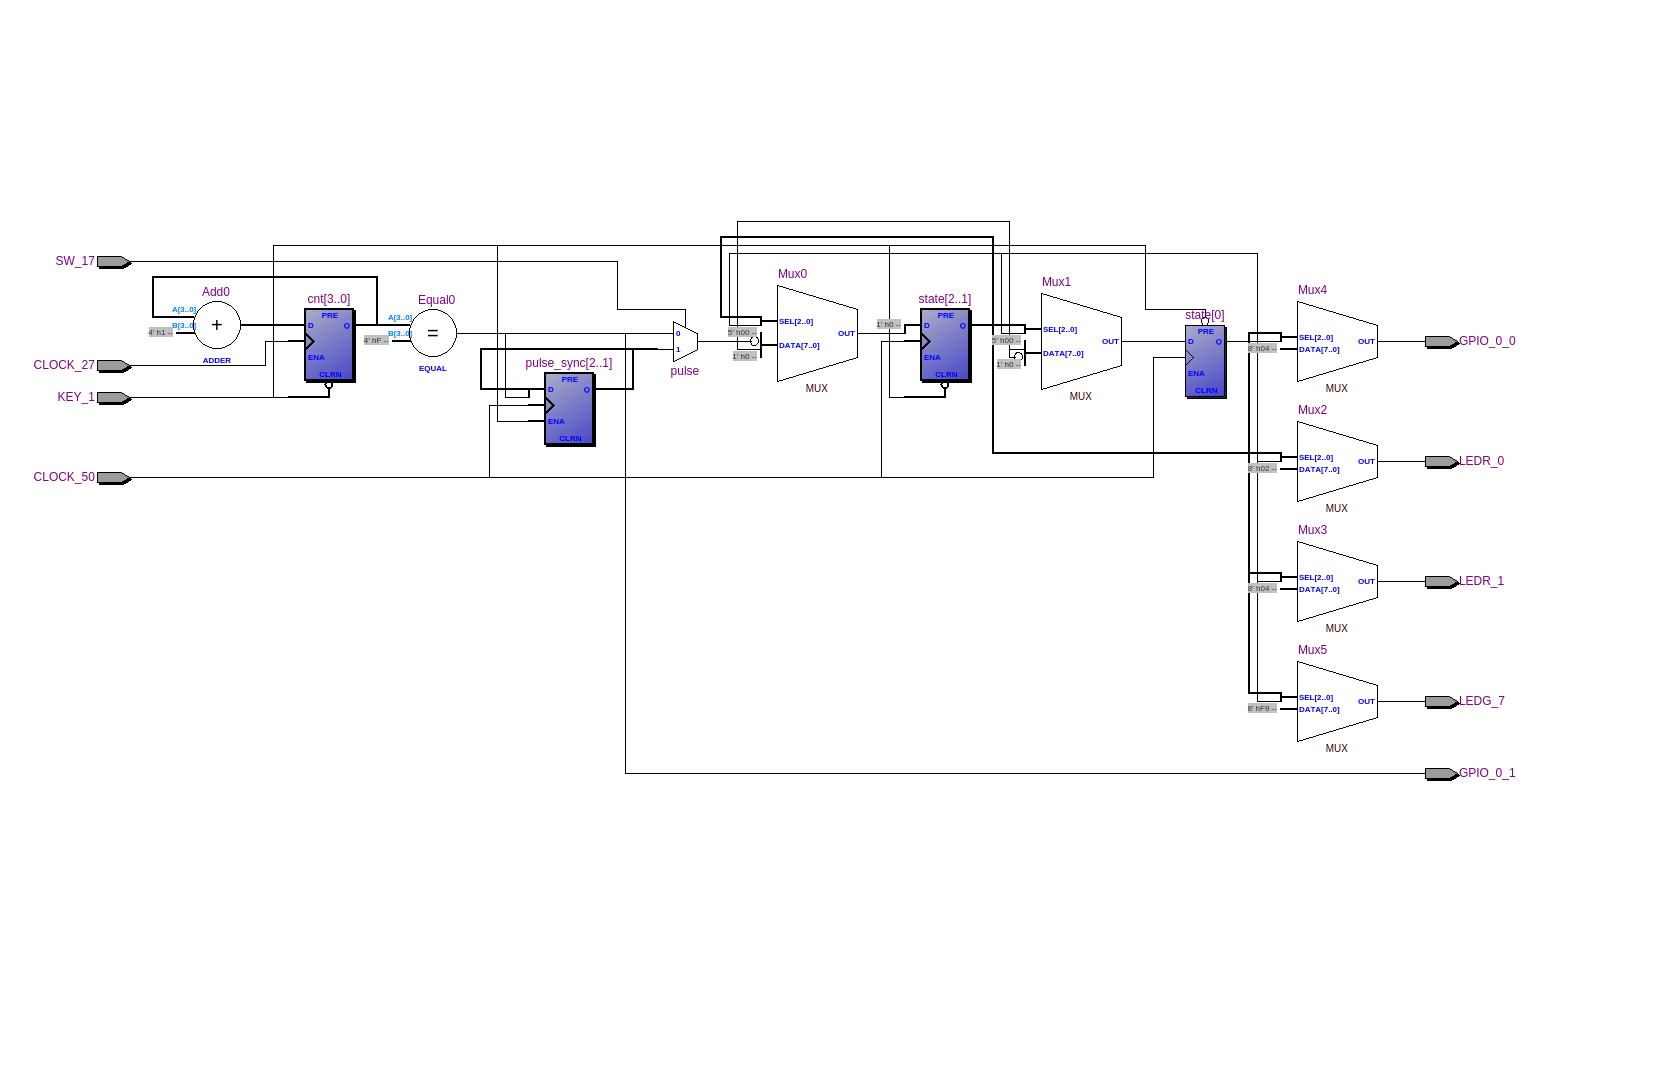
\includegraphics[width=1\textwidth]{images/metastability/RtL_metastaibility.png}
	\caption{RTL mit Synchronisations-Switch}
	\label{fig.metastabil.RtL}
\end{figure}

\newpage
\section{Resultat Metastabilität provozieren}\label{sect.meatastabil_proozieren}

Das Resultat ist, dass das Board unmittelbar nach Einstellen in den metastabilen Zustand fällt und die grüne LED leuchtet. Wird Reset gedrückt, folgt ein kurzes Aufblinken der zwei roten LEDs und wieder die grüne LED.

\begin{figure}[H]
	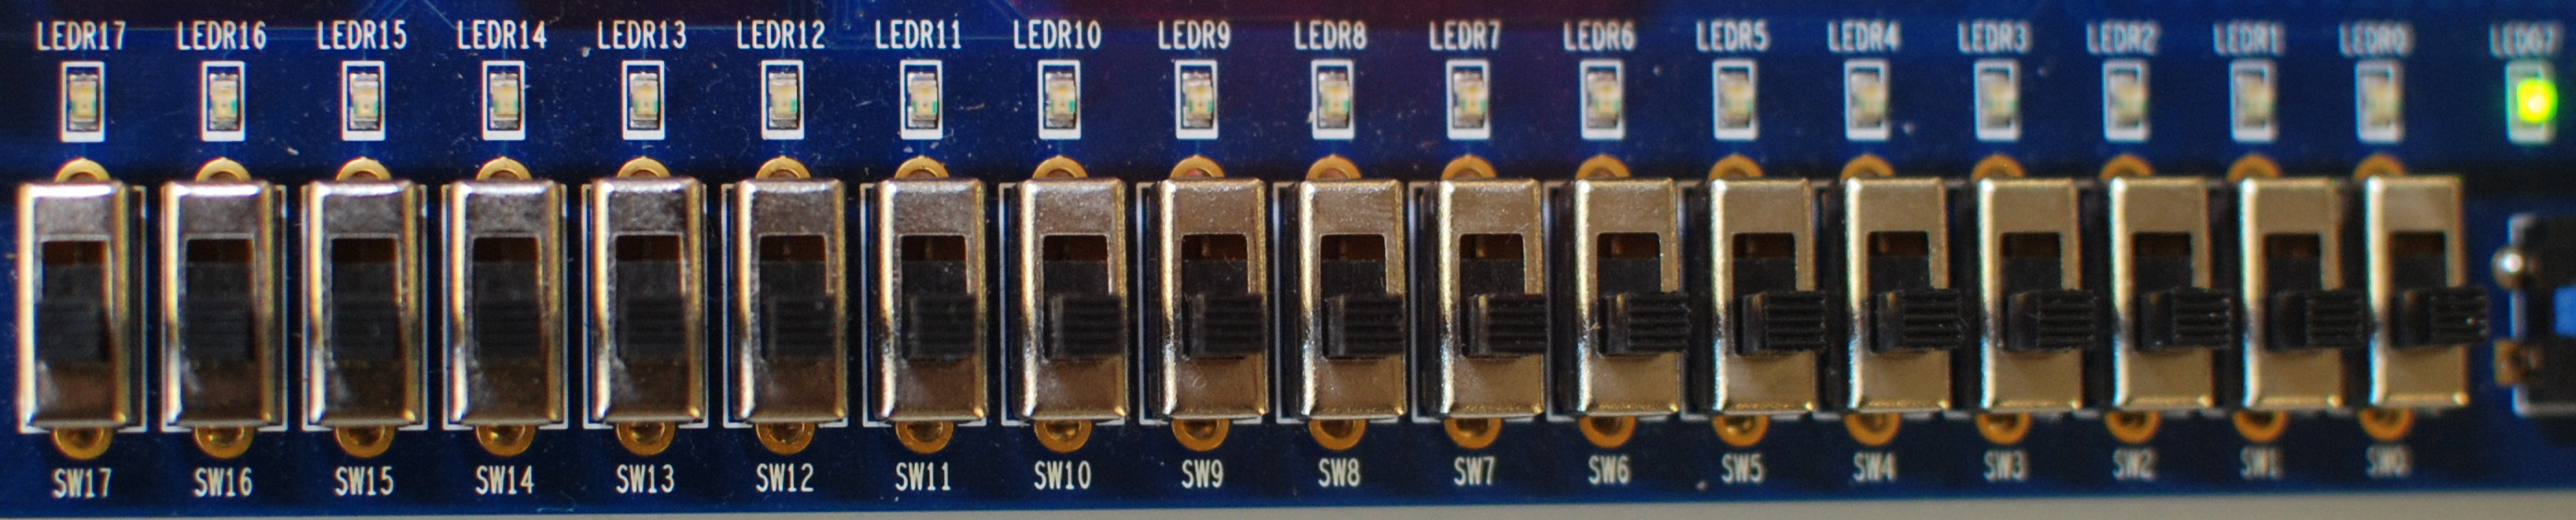
\includegraphics[width=1\textwidth]{images/metastability/metastabil.JPG}
	\caption{Metastbiler Zustand}
	\label{fig.metastabil.Ergebnis_Boardasynchron}
\end{figure}

Wird die Synchronisations-Schaltung betätigt, leuchten beide roten LEDs auf. Die \textit{fsm} wechselt zwischen den states s0 und s1 hin und her. Das Verbleiben in den zwei definierten Zuständen s0 und s1 funktioniert auch nach einem Tag noch.

\begin{figure}[H]
	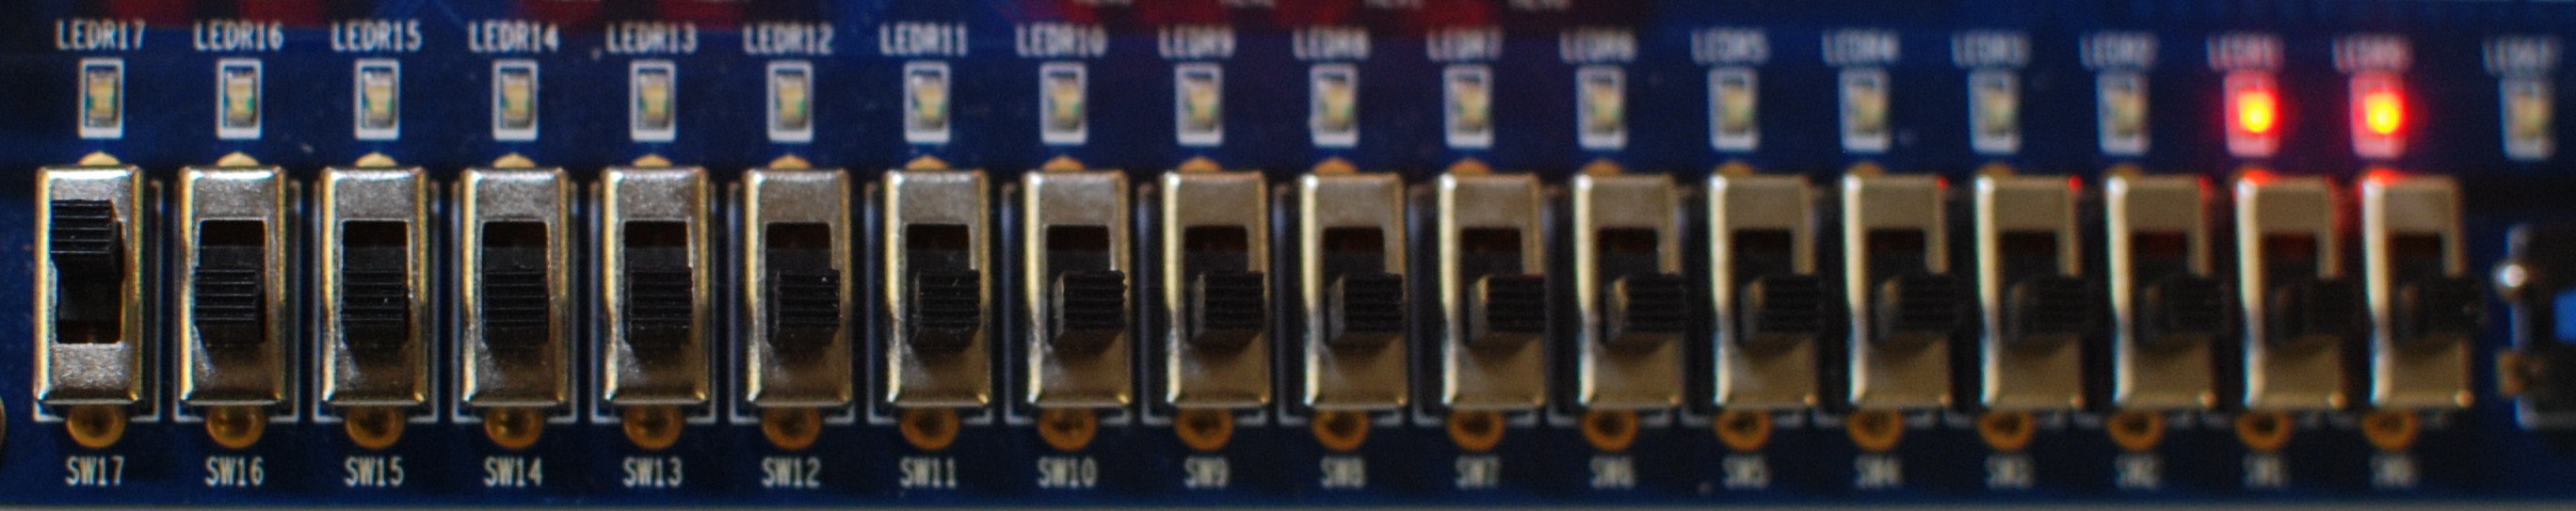
\includegraphics[width=1\textwidth]{images/metastability/synchronized.JPG}
	\caption{Switchschalter ON: Rote LEDs leuchten}
	\label{fig.metastabil.Ergebnis_BoardSynchron}
\end{figure}

\newpage
Wird das Wechseln zwischen den zwei states am KO ausgegeben, so erkennt man, da - weil der Takt 27 MHz kein Bruchteil von 50 Mhz - kein wiederkehrendes Muster der Wechsel zwischen den zwei Zuständen auftritt.

CH 1 = Rote LED\\
CH 2 = Synchronisierter Puls

\begin{figure}[H]
	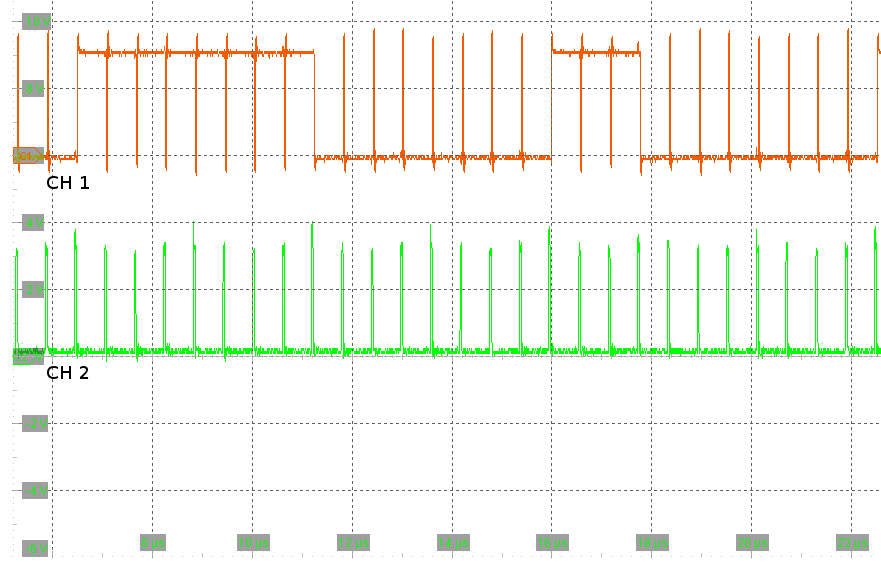
\includegraphics[width=0.8\textwidth]{images/metastability/synchron_eng_2.png}
	\caption{Erster Teil des unregelmässigen Wechsel zwischen Zustand s0 und Zustand s1}
	\label{fig.metastabil.Ergebnis_1}
\end{figure}

\begin{figure}[H]
	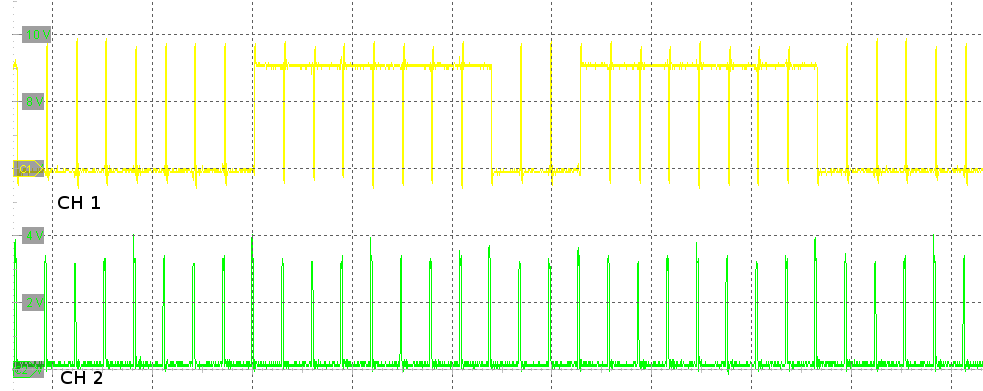
\includegraphics[width=0.8\textwidth]{images/metastability/synchron_eng_3.png}
	\caption{Zweiter Teil des unregelmässigen Wechsel zwischen Zustand s0 und Zustand s1}
	\label{fig.metastabil.Ergebnis_2}
\end{figure}

\newpage
Im Zustand der Metastabilität sind die Pulse nicht synchronisier und die rote LED geht nicht an.

\begin{figure}[H]
	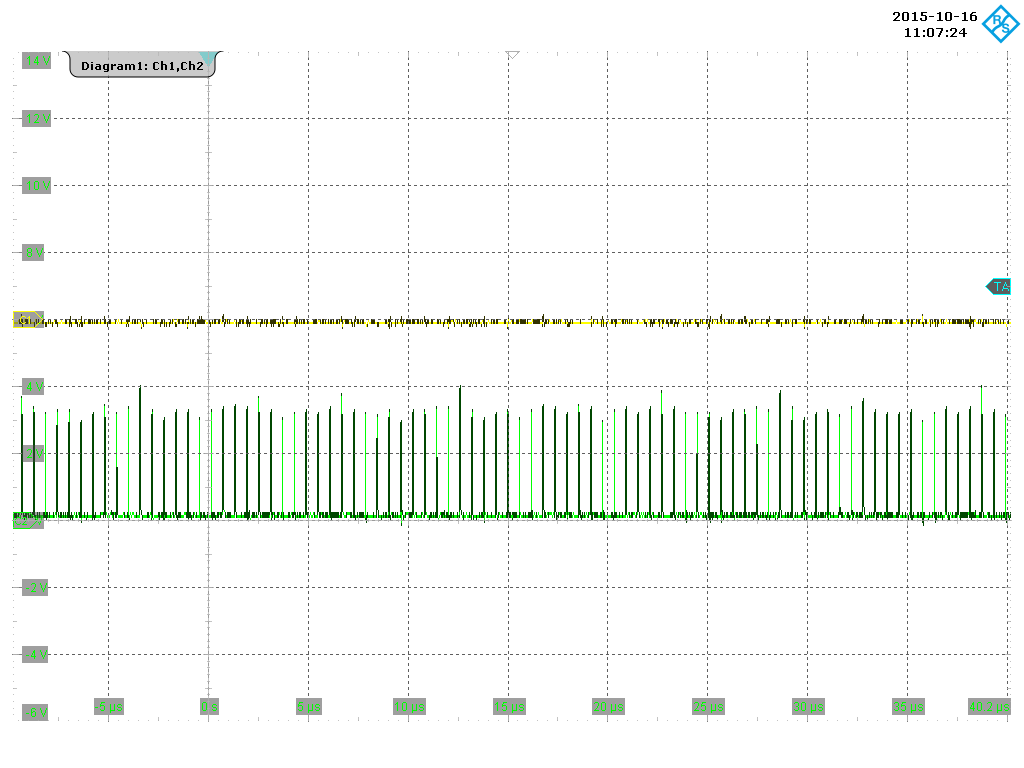
\includegraphics[width=0.8\textwidth]{images/metastability/asynchron_en_.png}
	\caption{Metastabiler Zustand}
	\label{fig.metastabil.Metastabil}
\end{figure}

